\chapter{Background and Literature Review} \label{chap:sota}

\minitoc \mtcskip \noindent

This section aims the analysis and reflection about some works that has as final goal, similarly to ours, the development of a framework with the purpose of exploring social media data to extract meaningful domain-specific information. Nonetheless, studying works from other authors may help or even find already proposed solutions in order to solve the aforementioned problems.

Hence, this section will contemplate a brief contextualization about how can an intelligent system contribute to the improvement of a \textit{smart city} or transportation services. Moreover, technologies and methods that allow extraction of information from a text document or, in this particular case, from tweets will be described. Finally, an exploration through already existent frameworks regarding the information extraction from social media content as well as the identification of its application domain.

\section{Smart Cities}\label{sec:smart_cities}

\textit{Smart City} is a concept appeared thanks to the continuous growth of a city's population which contributed to an aggressive level of urban and technological developments~\cite{kn:Cecilia2016}. In the last few years, several definitions for its meaning have emerged but its main idealization is not yet fully known~\cite{kn:Komninos2009}. Angelidou~\cite{kn:Angelidou2015} defined Smart City as

\emph{"Conceptual urban development model on the basis of the utilization of human, collective, and technological capital for the development of urban agglomerations"},

enhancing \textit{knowledge} and \textit{innovation economy} as the primary factors that support the development of a city. Alongside with the previous factors, the author identifies other three distinct forces that shape the concept of a \textit{smart city}:

\begin{enumerate}
	\item \textit{Technology Push}: The need of new products and solutions are introduced into the market due to a fast advance in science and technology.
	\item \textit{Demand Pull}: Current problems are solved originating new possibilities to respond society demands such as the continuous growth of the population.
	\item \textit{Urban Future}: Represents the final goal of a city constituting for that reason an important role in the whole transformation process.
	\item \textit{Knowledge and Innovation Economy}: The creation of new products using the most recent technologies is associated to solution for the efficiency and sustainability of a city.
\end{enumerate}

The first two forces previous mentioned are directly dependent of the other ones as it is showed in Figure~\ref{fig:four_forces}. However, the absence of desire to reach a better future having into consideration the city's economy and resources can result in the break of its dynamics and healthy, affecting services of a city due to the population discontentment.

\begin{figure}
	\centering
	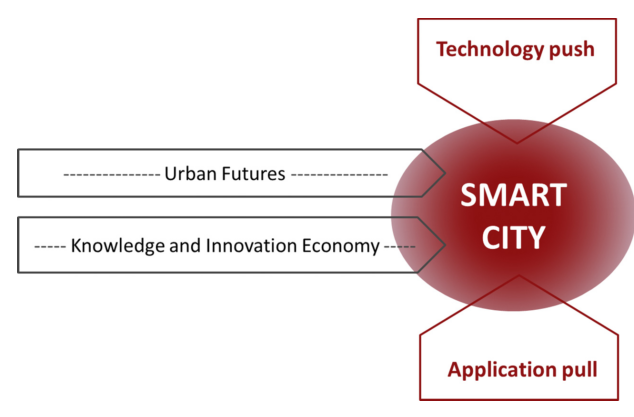
\includegraphics[width=0.6\textwidth]{figures/four_forces.png}
	\caption{\textit{Smart City} conjecture of four forces. Source:~\cite{kn:Angelidou2015}}
	\label{fig:four_forces}
\end{figure}

The development environment of a city tagged as \textit{smart} is another key factor to reach the success. Komninos~\cite{kn:Komninos2009} associates collective sources of innovation to the improvement of life quality in cities. The globalization of innovation networks is responsible for the emergency of another types of environments and infrastructures, as so \emph{"global innovation clusters and i-hubs, intelligent agglomerations, intelligent technology districts and intelligent clusters, living labs"} allowing the testing of products or services by the ordinary citizens in order to identify problems or even analyse their behaviour  and reactions regarding what have experimented~\cite{kn:Komninos2009}. Hence, it is possible to affirm that the development of a city has its starting point in the community but also depends on the quality of \glspl{ICT}~\cite{hollands2008will}, an essential requirement in the city's evolution process.

Last but not least, a \textit{smart city} may focus its efforts in several sectors, such as the environment, culture and recreation, education, social and economic aspects, demography, and travel and transportation~\cite{caragliu2011smart} in order to have equally advances in all of them.

\section{Intelligent Transportation Systems}\label{sec:intelligent_transportation_systems}

The transportation system is inherently connected to the progress of a city because people uses on a daily-basis transportation modes, i.e. bus, private cars, metropolitan, and others, in order to go to their jobs and make their own life and through that they contribute to the economic progress of it. Although this connection, such system is also influenced by the problem of population growth being relevant and necessary the finding of solutions to minimize or even erase it~\cite{kn:Caragliu2015}. Hence, "a \textit{smart city} should be focused on its actions to become smart", coming up the concept of innovation~\cite{kn:Cecilia2016}.

To understand what are \gls{ITS}, it is necessary to introduce the meaning of \gls{SM}. \gls{SM} is a combination of comprehensive and smarter traffic service with smart technology, enabling several intelligent traffic systems which provide control in the signals regarding the traffic volume, information about smooth traffic flows, times of bus, train, subway and flight arrivals, their routes or even the knowledge of what citizens thought about the city's services~\cite{kn:Chun2015}. The majority of \gls{ITS} are expressed through smart applications where transportation and traffic management has became more efficient and practicable, allowing the users to access important information about the transportation systems in order to make correct decisions about what they want to use in their cities~\cite{kn:Caragliu2015}. \gls{ICT}-based infrastructures are the main support for \textit{smart cities} and due to tha, they also serve as support to \gls{ITS}, since the information provide by such infrastructures allows the piloting of activities such as traffic operations, as well as its  management over a long period of time~\cite{kn:Cecilia2016}.

Nowadays, cities are exploring some initiatives of sensing to support the development of technological projects. Areas such as utilities management (where, for example, is monitored the consumption level of power, water and gas), traffic management (using vibration sensors to measure the traffic flows on bridges, or even the full capacity of a parking lot), environment awareness (using video cameras to monitor the population behaviour and sensors to measure the level of air pollution) make use of physical sensors, i.e. some devices that can capture information to study and improve the quality of life in a daily basis~\cite{kn:Doran2015}. Szabo et al.~\cite{kn:Szabo2013} and Doran et al.~\cite{kn:Doran2015} reported the highly economic cost to this kind of sensing, since it is require maintenance and replacement of this devices, as well as a tracking infrastructure to store and process the collected information. Hence, a new form of sensing has emerged - \gls{Crowdsensing} - offering to the cities several ways to improve their services by exploring the participation of the citizens through social networks where there is a publicly sharing of  opinions and thoughts regarding some problems around the city where they live are passing in~\cite{kn:Roitman2012}. This type of sensing consists in human-generated data provided by the population through the usage of mobile devices and social networks web-based platforms. Such data can be further used to extract some analytics regarding specific services in a city, namely the urban transportation system~\cite{kn:Roitman2012}. Having this considered, social media can be seen as a good source of data to extract valuable information aiming the direct use of it into the smartness evolution process of a city~\cite{kn:Szabo2013}. Recently, it is possible to verify that cities are increasingly opting for technological opportunities based on \textit{crowd sensing}, once this type of exploration brings a considerable reduction of costs and support in the development of news valuable technologies.

In the last few years, several authors have published a widely range of social-media-based contributions focusing this specific domain. Kurkcu et al.~\cite{kurkcu2016evaluating} use geo-located tweets to try and discover human mobility and activity patterns. The subject of transport modes was explored by Maghrebi et al.~\cite{maghrebi2016transportation} in the city of Melbourne, Australia. From a dataset of 300,000 geo-located tweets, authors tried to extract tweets related to several modes of transport using a keyword-based search method. 

Additionally, there were also different efforts focused on the tracking of accidents using Twitter social media data. Mai and Hranac~\cite{mai2013twitter} tried to establish a correlation between the California Highway Patrol incident reports and the increased volume of tweets posted at the time they were reported. On the other hand, Rebelo et al.~\cite{rebelo2015twitterjam} implemented a system capable of extract and analyse events related to road traffic, coined  TwitterJam. In that study, authors also used geo-located tweets that were already confirmed as being related to events on the roads and compared their counts with official sources.

Performing robustness experiments over this domain is challeging since although the large number of recently publications, gold standards are yet not defined or even public being for this reason difficult to prove the methodology chosen or suppositions made. Maghrebi et al.~\cite{maghrebi2016transportation} enhances some terms related to the transportation domain, however they are limited and also very common ones. After a tough investigation work, it is worth noting a list produced by Gal-Tzur et al.~\cite{gal2014potential} containing a large number of terms whose may serve as support for new  scientific contributions using social media in studies of the transportation domain.

\section{Social Media Analytics}

In the last few years social networks have made impact on the business communications since users assumed the role of costumers through the publication of content on these networks, rising high levels of interaction between them, as well as with businesses entities~\cite{kn:Cecilia2016}. A proof of that is the amount of information produced since 2011 which is equivalent to a number over than 90\% of the available data online~\cite{kn:SINTEF}. Facebook\footnote{\url{https://www.facebook.com/}}, Twitter\footnote{\url{https://twitter.com/}} and other social networking websites are nowadays used as business tools by companies aiming the efficient use of digital marketing techniques to publicize their products~\cite{kn:Royle2014}. Besides the business field, the population turn widely into this new communication technologies publicly sharing real-life events, their opinions about certain topics and their on-time feelings in the network through a simple message \cite{kn:DAndrea2015}.

Social Media Analytics (SMA) can be described as a type of digital analytics which focus is the study of interactions between, their opinions/thoughts, their own life, companies as so its products or services through the social media data. Such study provides important information to "analysts, brands, agencies or vendors" facilitating the generation of economic value to many organizations~\cite{kn:Judah2012}. In order to achieve the main goal of the SMA, companies focus their effort in the development automatic systems to make possible an easy collection, analysis, summarization and visualization of processed social media data establishing specific points about what is necessary to improved in their products~\cite{zeng2010social}.

However the potential value that SMA can provide, Phillips~\cite{kn:Judah2012} enhance some important factors to be considered in the analytics process: (1) Users permissions; (2) Awareness/listening of real-time information; (3) Search mechanisms; (4) Text analysis methodologies and techniques; (5) Data access and integration; (6) System integration, customization and growth.

The previous mentioned factors will help during the identification and comprehension of possible necessary features in a social media analytics tool, as well as to establish potential parameters/metrics to test and evaluate such tool. Without careful conduction in the social media tool elaboration, for instance, use of a wrong technique of SMA could have a bad business impact for the company resulting possible bankruptcies and increase the unemployment tax of a city.

%\subsection{Data Management}
%\subsection{The potential of Twitter}

\section{Text Mining}

Text mining is a conjecture of fields such as information retrieval, data mining, machine learning, statistics and computational linguistics which aims the extraction of valuable information from unstructured textual data~\cite{kn:He2013}. The intensively usage of this analysis methodology is due to the massive amount of information stored in text documents being necessary automatic techniques to identify, extract, manage and integrate the knowledge acquired from these texts exploration in a efficiently and systematically way~\cite{ananiadou2015textmining}. On the other hand, the emergency of social media applications have also contributed to the widely growth of text mining usage because of the "application’s perspective and the associated unique technical and social science challenges and opportunities"~\cite{zeng2010social}.

Text mining shares some of the issues presented by the Natural Language Processing (NLP) field. Texts are usually performed by humans and due to that, some problems in its construction can appear, such as spelling mistakes, wrong phrasal construction, slang among other. Before the mining process of a text, it's important to apply some preprocessing steps in order to eliminate or, at least reduce, undesired content (words) in the primary analysis process.
A. Stavrianou et al.~\cite{kn:Stavrianou2007} cite these issues very well alongside their work and some of them are observable in Table~\ref{table:textminingissues}.

\begin{table}[htbp]
	\centering
	\caption{Text mining issues by Stavrianou \cite{kn:Stavrianou2007}}
	\label{table:textminingissues}
	\begin{tabular}{ | l | p{7cm} |}
		\hline \textbf{Issue}            & \textbf{Details}\\
		\hline Stop list                 & Should we take into account stop words?\\ 
		\hline Stemming                  & Should we reduce the words to their stems?\\ 
		\hline Noisy Data                & Should the text be clear of noisy data?\\ 
		\hline Word Sense Disambiguation & Should we clarify the meaning of words in a text?\\ 
		\hline Part-of-speech Tagging    & What about data annotation and/or part of speech characteristics?\\ 
		\hline Collocations              & What about compound or technical terms?\\ 
		\hline Grammar / Syntax          & Should we make a syntatic or grammatical analysis? What about data dependency, anaphoric problems or scope ambiguity?\\ 
		\hline Tokenization              & Should we tokenize by words or phrases and if so, how?\\ 
		\hline Text Representation       & Which terms are important? Words or phrases? Nouns or adjectives? Which text model should we use? What about word order, context, and background knowledge? \\ 
		\hline Automated Learning        & Should we use categorization? Which similarity measures should be applied? \\ \hline
	\end{tabular}
\end{table}

The removal of words from text may sometimes not be desirable because some sentences can lose its information or even leads to a different meaning compared with its original form. The generation of a stop list words should be a supervised task as long as little words could induce distinct results in the text classification~\cite{kn:Riloff1995}.

Stemming is a task that depends mostly from the speaking language of the text than its specific domain~\cite{kn:Stavrianou2007}. The main goal of this technique is to reduce a word to its root form helping in the calculus of distances between texts, keywords or phrases, or even in the text representation.

The noisy data is derived from spelling mistakes, acronyms and abbreviations in texts and to solve this, a conversion of these terms should be done to maintain the integrity of data. Commonly solution approaches involve text edit distances (Levenshtein Distance\footnote{\url{https://en.wikipedia.org/wiki/Levenshtein_distance}}) and phonetic distances measures between known words and the misspelling ones to achieve good corrections~\cite{kn:Bontcheva2013} 

Word Sense Disambiguation (WSD) focus on solving the ambiguity in the meaning of a word. Other similar field to WSD is Name Entity Disambiguation (NED) where the disambiguation target are named-entities mentions, while WSD focus on common words. WordNet\footnote{\url{https://wordnet.princeton.edu/}} is a commonly used resource to extinguish this ambiguity \cite{kn:Chang2016}. There are two types of disambiguation: the unsupervised, where the task is support by a dictionary or a thesaurus \cite{kn:Stavrianou2007}; and, the supervised one, where different meanings of a word are unknown and normally learning algorithms with training examples are used to achieve good results regarding the performance of the disambiguation task~\cite{kn:Yarowsky1995}.

Tagging can be describe as the process of labeling each term of the text with a part-of-speech tag, i.e. classify each word as a noun, verb, adjective, and others \cite{kn:Hotho2005}. Collocations are groups and constitutes a very important step in some text mining approaches. Grouping two or more words to give its correct meaning is sometimes crucial to perform tasks such as sentiment analysis where negations (e.g. "don't like") needed to be composed by two or more words in order to assure the negative value of, for example, a verb. Collocations are usually made before the WSD task since some compound technical terms have different meaning from the individual words which composed it \cite{kn:Stavrianou2007}.

Tokenization serves to pick up all the terms presented in a text document and to achieve this it's necessary splitting its content into a stream of words implying the removal of the punctuation marks and non-text characters \cite{kn:Hotho2005}. Some authors also see tokenization as a text representation form since one of the most used models to represent texts is \textit{Bag-of-words} (BoW). This model broke down texts into words and stores it in a term-frequency vector according the occurrence of a word in the text. Hence, each word may represent a feature \cite{kn:Sriram2010}. Another commonly used model to represent texts is Vector Space Models that represent all the documents in a multi-dimensional space where documents are converted to vectors and each vector may be seen as a feature. This model provides some advantages since the documents can be compared with each other by performing some specific vector operations \cite{kn:Hotho2005}.

Once been introduced some of the most preliminary important steps in text mining, the remainder subsection are focused in two different text analytics approaches: topic modelling and text classification. The majority of Social Media Analytics approaches focus its efforts in modelling and classification tasks in order to understand the large range of data collected and support commonly used techniques to extract information from it, such as sentiment analysis, trend analysis and topic modeling~\cite{kn:Fan2013}.

\subsection{Topic Modelling}
\label{subsec:topic_modelling_sota}

Topic modelling is a text mining unsupervised technique/method aiming the identification of similarities in unlabeled texts. Usually, this technique is applied over texts of large volume since to correctly identify the resulting patterns in its content requires the existence of lots of information.

One of the first studies made using Twitter data was proposed by Kwak et al.~\cite{kwak2010twitter} and consisted in the collection of messages to classify the trends in its content. Results showed that almost 80\% of the trends in Twitter are related to real-time news and the period in which each trend maintains itself in the top is limited. The authors proved that Twitter can be seen as a mirror of real-time occurring events/incidents in the world.

Several works were already proposed to identify social patterns in the population daily-basis life and mapping such patterns geographically by topic modelling techniques to discover latent topics in social media streams. Usually, studies about topic modelling, in particular \gls{LDA} model, to text mining problems follow unsupervised approaches~\cite{lansley2016geography,oliveira2016sentibubbles} - where is not required the creation of a training dataset. Others improved the model and made it an supervised approach~\cite{ramage2010characterizing}, dependent of training data, and compare to the traditional one in order to prove better results.

Using entity-centric aggregations and topic modelling techniques, Oliveira et al.~\cite{oliveira2016sentibubbles} built a system focused in data visualization that allows an user to search for an entity during a specific period and shows which are the main topics identified in the Twitter messages.  Ordinary weekday patterns were identified by Lansley et al.~\cite{lansley2016geography} in their study regarding the inner region of London. The authors used a \gls{LDA} model to distribute 20 topics over 1.3M tweets. After crossing the results of the experiment with land-uses datasets it was possible to observe interesting patterns in specific zones and places of the British city. Nonetheless, Ramage et al.~\cite{ramage2010characterizing} improved a \gls{LDA} model by adding a supervised layer that automatic label each tweet used in their experiment.

\gls{CRF} are explored by Nikfarjam et. al~\cite{nikfarjam2015pharmacovigilance} which have applied word embeddings in combination to other text features, such as adverse drug reactions lexicons, \gls{POS} and negation collocations in order to train a supervised model. Such model was able to demonstrate high performances on the extraction of concepts/topics from the social media user-generated content. To prove robustness and efficiency in the model, authors have compared the obtained results with DailyStrength corpus and were able to notice that due to the limited size of text in a tweet, the detection of different reactions about drugs is more complex, which could be simplified with access of greater amount of information provided in the training process of the model.

Differently from the majority of works involving topic modelling techniques, Tuarob and Tucker~\cite{tuarob2015quantifying} take support of a \gls{LDA} model to extract the most frequent words for groups of tweets previously collected. The overall work is focused in sentiment analysis approaches and aims the perception of what people fells about a specific product as well as its composing features. Authors used the \gls{LDA} model to find what were the main 2 topics present in each product set of tweets and considered the most frequent 30 words. Moreover, POS tagging, disambiguation and stemming techniques were used in order to filter out and normalized words related to the product. Finally, an unsupervised method to calculate the sentiment polarity was applied to the data being final results coherent to the product feature/aspect extracted.

Topic modeling techniques consisting in supervised learning approaches were explored by Zhang et al.~\cite{zhang2016mining}, where authors have compared the results obtained from a SVM classification for accident-related tweets with a classification using a two-topic generative model SLDA (Supervised \gls{LDA}). Contrarily to the unsupervised method, this one takes into consideration the label assigned to the training examples and can be trained as a genuine classification model. By comparing the final results between both models, it is possible to observe a significative increase of the precision and a decrease of only 0.04 points in the accuracy meaning that supervised topic modelling techniques to binary classification may compete well with conventional classification models, with respect to tweets.

\begin{table}[htbp]
	\centering
	\caption{Brief overview of the related work for topic modelling}
	\label{tab:topic_related_work}
	\resizebox{\textwidth}{!}{\begin{tabular}{c|c|c|c|c}
			\hline
			\textbf{Approach} & \textbf{Features} & \textbf{Methods} & \textbf{Goal} & \textbf{Potential Domain}\\ \hline
			H. Kwak et al.~\cite{lansley2016geography} & Twitter metadata & \begin{tabular}[c]{@{}c@{}} Aggregation of trending topics using \\external information \end{tabular} & \begin{tabular}[c]{@{}c@{}} Quantitative study in order to reveal Twitter\\ as both social media and news media platform \end{tabular} & Smart City \\ \hline
			
			J. Oliveira et al.~\cite{oliveira2016sentibubbles} & specific-entity words & \begin{tabular}[c]{@{}c@{}}Unsupervised Latent Dirichlet \\ Allocation\end{tabular} & \begin{tabular}[c]{@{}c@{}} Extract the most relevant entity-related topics \end{tabular} & Smart City \\ \hline
			
			G. Lansley and P. Longley~\cite{lansley2016geography} & Bag-of-words & \begin{tabular}[c]{@{}c@{}}Unsupervised Latent Dirichlet \\ Allocation\end{tabular} & \begin{tabular}[c]{@{}c@{}} Study social dynamics of London using Twitter topics\end{tabular} & Smart City \\ \hline
			
			S. Tuarob and C. Tucker~\cite{tuarob2015quantifying} & Bag-of-words & \begin{tabular}[c]{@{}c@{}}Unsupervised Latent Dirichlet \\ Allocation\end{tabular} & \begin{tabular}[c]{@{}c@{}} Extraction of people's polarization sentiment about a\\ specific feature of a product (aspect sentiment analysis)\end{tabular} & Smart City - Economy \\ \hline
			
			D. Ramage et al.~\cite{lansley2016geography} & Labeled bag-of-words & \begin{tabular}[c]{@{}c@{}}Supervised Latent Dirichlet \\ Allocation\end{tabular} & \begin{tabular}[c]{@{}c@{}} Proving the applicability of supervised approaches\\ in conventional \gls{LDA} model \end{tabular} & Smart City \\ \hline
			
			Z. Zhang et al.~\cite{zhang2016mining} & Labeled bag-of-words & \begin{tabular}[c]{@{}c@{}}Supervised Latent Dirichlet \\ Allocation~\cite{mcauliffe2008supervised}\end{tabular} & \begin{tabular}[c]{@{}c@{}} Comparing performances with SVMs models \\ to accident-related tweets \end{tabular} & \begin{tabular}[c]{@{}c@{}}Smart City - Travel and \\Transportation\end{tabular} \\ \hline
			
			A. Nikfarjam et. al~\cite{nikfarjam2015pharmacovigilance} &  \begin{tabular}[c]{@{}c@{}}ADR Lexicons, POS Tagging \\ Negation, Word Embeddings\end{tabular} & CRF & 
			\begin{tabular}[c]{@{}c@{}} Discrimination of adverse drug reactions in tweets\\ content\end{tabular} & Smart City - Health \\ \hline
		\end{tabular}}
	\end{table}
	
Probabilistic topic models, such as \gls{LDA}, are the most used techniques in topic detection tasks. Although high applicability, authors question themselves regarding the performance of this technique over social media data which present limitations, starting at the size of the message and ending in the bad phrasal construction and informality~\cite{kn:Mehrotra2013}. In this dissertation we will tackle this question and try to answer it by presenting results obtained in a real-world scenario experiments.

\subsection{Text Classification}

Text classification is a text mining task which main goal is the discrimination or characterization of a piece of text into a specific format value. Such value can vary from number (sentiment analysis tasks), labels (multi-labeling tasks), classes (binary or multi-class tasks). Classification in text analysis is a widely used methodology and had already been reported in several scientic contributions regarding the smart cities and transportation domains.

\gls{SVM}, \gls{OLS}, \gls{RF}, \gls{MLP}, \gls{NB} and \gls{DT J48} are some of the supervised classification models used to analyse social media data over fields such as health~\cite{signorini2011use} and pharmacovigilance, political opinion~\cite{saleiro2016sentiment}, transportation (travel classification~\cite{carvalho2010real, kuflik2017automating}, traffic and incidents detection~\cite{zhang2016mining}), financial sentiment analysis~\cite{saleiro2017feup} and \textit{online} reputation monitoring~\cite{saleiro2017texrep}.

Sifnorini et al.~\cite{signorini2011use} reported a study which main goal was the tracking of the disease \gls{Influenza_A} virus. Tweets collected by the authors using term-based search sum up more than 300 million examples. Their methodology consists in training \gls{SVM} models with sets of frequency features composed by the most used weekly-terms over the whole dataset. Each model was specifically trained according a certain set of keywords and follow an iterative process, i.e. authors firstly have classified all illness-related tweets related and than used the resulting related subset of data to perform new classification regarding specific keywords, such as what was the disease source, countermeasures used and infected people characteristics. Final results allowed the verification of a decrease of Twitter activity while more new cases were appearing meaning less concerning about this epidemic through time.

Accident-related classification for Twitter data was proposed by Zhang et al.~\cite{zhang2016mining}. Authors explored the Twitter Streaming API to collect geo-located tweets from Northern Virginia during a completed year, January to December of 2014, and recurring to auxiliary loop detectors that are, in intervals of 15 minutes, recording the traffic flow. In order to automatize the detection of accidents in that interval of time (were the sensors are not recording the scene), authors have built a binary classification model using Linear \gls{SVM} with a balanced dataset composed by 400 training examples for each of the accident-related and non-related classes composed by a boolean-vectors according the final 3,000 tokens resulted from the token filtering and stemming process. Performance was improved by submitting the model to a 5-fold cross validation which was proved by values of accuracy and precision over than 70\% of success.

%J. Pereira et al.~\cite{pereira2017transportation} try to discriminate travel-related tweets recurring to a combination of two different types of features: bag-of-words and word embeddings. Authors explored almost 9,000,000 geo-located tweets from two Brazilian \textit{megacities} and construct, manually, a balanced training dataset of travel-related and non-related tweets. The binary classification proved to have better performance under the SVM model experiments with linear \textit{kernel} function, as well as the two previous mentioned works here.

Considering the task of discriminate travel-related tweets, Carvalho et al.~\cite{carvalho2010real} have constructed a bag-of-words dependent classification model and achieved improvements at the model's performance with support of a bootstrapping approach implying a two phases train to the \gls{SVM} model.  By assuming the similarities, i.e. all four works were related to binary text classifications, we can induce an hypotheses that Linear \gls{SVM} models have superior performances relatively to other models for this type of classification tasks.

Multi-class classification models were also applied to the transportation domain through text analysis of social media content. Kufliket et al.~\cite{kuflik2017automating} build multiple classification models using methods such as \gls{NB} and \gls{DT J48} to predict multiple modes of transport during three different sports events. Tweets sum up a total of 3.7M and were submitted to the models classification task in order to prove that an harvesting automatically information from \gls{SMC} is possible and may help transportation entities in the planning and management of their services during social occasions as it is demonstrate in theirs use cases.

On the other hand, Saleiro et al.~\cite{saleiro2016sentiment} tried to predict the 2011 Portuguese bailout results analysing opinion within the tweets about all five political parties candidates. The opinion was measure using a \gls{OLS} model trained with specific sentiment aggregate functions and proved to be capable of correctly predict who would be elected prime minister of Portugal only exploring sentiment analysis in social media data. In SemEval-2017 Task 5, Saleiro et al.~\cite{saleiro2017feup} explored word embeddings techniques to extract the sentiment polarity and intensity in financial-related tweets. Authors have proved good performance of models trained with bag-of-words and bag-of-embeddings features together although the approach been applied to a specific domain. The usage of features representing syntactic and semantic similarities of texts, such as word embeddings, can be seen with great potential namely to the area of travel-related text classification.

\begin{table}[htbp]
	\centering
	\caption{Brief overview of the related work for text classification - Best Experiments}
	\label{my-label}
	\resizebox{\textwidth}{!}{\begin{tabular}{c|c|c|c|c}
			\hline
			\textbf{Approach} & \textbf{Features} & \textbf{Classification Methods} & \textbf{Goal} & \textbf{Potential Domain}\\ \hline
			Sifnorini et al.~\cite{signorini2011use} & Bag-of-words & Linear SVM & \begin{tabular}[c]{@{}c@{}}Tracking the evolution of public sentiment\\ and increasing of social media activity about\\ the H1N1 pandemic\end{tabular} & Smart City - Health \\ \hline
			
			Zhang et al.~\cite{zhang2016mining} & \begin{tabular}[c]{@{}c@{}}Boolean vectors matrix \\ (3,000 different tokens)\end{tabular} & Linear SVM & \begin{tabular}[c]{@{}c@{}}Improve transportation control by automatic \\discriminate accident-related tweets \end{tabular} & \begin{tabular}[c]{@{}c@{}}Smart City - Travel and \\Transportation\end{tabular} \\ \hline
			
			%J. Pereira et. al~\cite{pereira2017transportation} &  \begin{tabular}[c]{@{}c@{}}Word Embeddings,\\ Bag-of-words\end{tabular} & Linear SVM & \begin{tabular}[c]{@{}c@{}} Discrimination of travel-related tweets through \\word embeddings techniques\end{tabular} & \begin{tabular}[c]{@{}c@{}}Smart City - Travel and \\Transportation\end{tabular} \\ \hline
			
			Kuflik et al.~\cite{kuflik2017automating} & Bag-of-words &  \begin{tabular}[c]{@{}c@{}} Naïve Bayes, \\ DT J48\end{tabular} & \begin{tabular}[c]{@{}c@{}}Multi-class mode of transport classification and the \\ purpose behind it\end{tabular} & \begin{tabular}[c]{@{}c@{}}Smart City - Travel and \\Transportation\end{tabular} \\ \hline
			
			Carvalho et al.~\cite{carvalho2010real} & Bag-of-words & \begin{tabular}[c]{@{}c@{}}Linear SVM with \\ Bootstrapping\end{tabular} & Discrimination of travel-related tweets & \begin{tabular}[c]{@{}c@{}}Smart City - Travel and \\Transportation\end{tabular}\\ \hline
			
			Saleiro et al.~\cite{saleiro2016sentiment} & \begin{tabular}[c]{@{}c@{}} Sentiment Aggregate\\ Functions \end{tabular} & OLS & \begin{tabular}[c]{@{}c@{}} Predicting Portuguese polls results through \\ opinion mining \end{tabular} & Smart Cities - Government \\ \hline
			
			Saleiro et al.~\cite{saleiro2017feup} & \begin{tabular}[c]{@{}c@{}}Word Embeddings,\\ Bag-of-words,\\ domain-specific lexicons\end{tabular} & RF & \begin{tabular}[c]{@{}c@{}} Extraction of sentiment polarity and intensity from social\\  media content and web news \end{tabular} &  Smart City - Economy \\ \hline
			
		\end{tabular}}
	\end{table}

\medskip

There is a wide diversity in text classification approaches. A worth noting fact in this review at the literature is that word embeddings have been supporting conventional techniques in order to improve performances in text classification tasks. Transportation domain lacks in studies having this particular feature in the training process of its classification models. Hence, it is of major importance perform experiments about this domain aiming conclusions and additional content to support the potential advantages brought by word embeddings.

\subsubsection{Classification Evaluation Metrics}
\label{subsubsec:evaluation_metrics}
In order to measure the performance of a text classification model, there are several types of metrics that can help this process, depending of course the context of the task. Regarding binary classification tasks, the most common evaluation metrics used are precision, recall (sensitivity) and F1-score which is the harmonic mean or the weighted average of the previous two. Therefore, it is described each of these metrics as well the mathematical equation used in its calculation.

\begin{itemize}
	\item \textbf{Precison:} Represents the fraction of correct predictions for the travel-related class (Equation~\ref{eq:precision}).
	
	\item \textbf{Recall:} Represents the fraction of travel-related tweets correctly predicted (Equation~\ref{eq:recall}).
	\begin{multicols}{2}
		\begin{equation}\label{eq:precision}
		Precision = \frac{tp}{tp+fp}
		\end{equation}
		
		\begin{equation}\label{eq:recall}
		Recall = \frac{tp}{tp+fn}
		\end{equation}
		\end{multicols}
		
		where \textbf{$tp$} is related to the true positives classified tweets, \textbf{$fp$} represents the false positives and \textbf{$fn$} are the false negatives.
		
		\item \textbf{F1-score:} Represents the harmonic mean of precision and recall.
		\end{itemize}
		
		\begin{equation}
		{F1}_{score} = 2*\frac{precision*recall}{precision+recall}
		\end{equation}
		
These first three metrics only showed us the performance of the classifier for a discrimination threshold of 0.5. The \gls{ROC} curve gives us the \gls{TPR} and the \gls{FPR} for all possible variations of the discrimination threshold. Through the \gls{ROC} curve, it is possible to compute the \gls{AUC} to see what was the probability of the classifier to rank a random positive higher than a random negative one.

\section{Related Social Media Frameworks}

In the last few years, the number of proposals of frameworks to treat social media content and produce valuable information to the end-users has widely increased. For instance, each framework has it own domain of application and generalization is not the center focus. Event detection, \textit{online} reputation monitoring, socio-semantic analysis to human reactions and traffic sensing are some of the application domains that research community present their contribute through framework proposals.

Liu et al. \cite{kn:Liu2012} have made a study in three different transportation modes (private cars, public transportations and bicyclists) using theirs channels on Twitter to estimate a percentage of the majority gender that uses this services in the city of Toronto. They have extracted all the channel's tweets appealing only to the \textit{non-protected} followers and applied an already developed classification model to label each tweet with its creator gender: male or female. Author decided to implement a system that produce automatically analysis since they have find interesting results in the experiment conducted.

Regarding the field of event/incident detection, Abel et al~\cite{kn:Abel2012} developed Twitcident, a real life accidents-aware web-based framework that is connected to a emergency broadcast system in order to detect incidents across the world. Then, an automatically system starts the collection and filtering of content from social media platforms and extracts information about entities using Named Entity Recognition and Disambiguation techniques. Data temporal distributions are also produced to analyse the time line of the events.

Anastasi et al. \cite{kn:Anastasi2013} proposed a framework which objective was the promotion of flexible transportation systems usage, i.e. encouraging people to share transport or to opt for the use of bicycles in order to minimize infrastructural and environmental problems. Their tool takes advantages of the crowd sensing techniques by exploring social media streams to predict accidents or traffic congestion and alert the users of their service about this type of events.

Ludwig et al. \cite{kn:Ludwig2015} proposed a tool capable of collect and display social media streams in order to help the integration and coordination of volunteers in actions performed by emergency services to prevent engagement in dangerous areas. Their tool present to the end-users map visualization of a city where they could identify public calls of the emergency services to accept or deny them.

Traffic sensing over the city of Rio de Janeiro, Brazil, was studied by Rebelo et al.~\cite{rebelo2015twitterjam} which have implemented a system capable of extract and analyse events related to road traffic, coined  TwitterJam. In that study, authors used geo-located tweets that were already confirmed as being related to events on the roads and compared their counts with official sources. Finally but not least, authors present interesting geographic visualizations to the end-users in order to understand what is the current traffic-state of a certain road.

Social Media is used by Ludwig et al.~\cite{kn:Ludwig2015}, in a framework that attempts the creation of voluntary and emergency activities, coined CrowdMonitor. The systems allows through the analyse of human mobality through tweets posted in the platform. Although absence of text analysis methodologies, such system intents to promote more cooperation between citizens and also promotes the applicability of crowd sensing, a crucial factor for the smartness evolution of a city.

Technological companies is the main target of the framework proposed by Lippizzi et al.~\cite{kn:Lipizzi2015}. The system analyses social media content having in consideration specific products, such as mobile phones, tablets and others, and tries to extract information of what their customers think and talk about it. By measuring the sentiment of word clusters produced by the system, companies may take profit and additional insights about what in needed to be improved in their products.

CrowdPulse is a domain-agnostic framework proposed by Musto et al.~\cite{musto2015crowdpulse} which main objective is the presentation of text analytics to the end-users. Such framework is rich regarding implemented text methods, which range from entities disambiguation to sentiment analysis. Authors followed unsupervised approaches to implement all the framework composing methods, and applied the resulting system in two real-world scenarios, the earthquake of L'Aquila city and The Italian Hate Map. Further analysis of the results proved that simple techniques can provide faster insights about people sentiment regarding any type of domain.

A full-based text mining framework for \textit{online} reputation monitoring is proposed by Saleiro et al.~\cite{saleiro2017texrep} cabable of explore and extract multiple types of information from a wide range of Web sources. TextRep is divided in several modules in order to perform correctly the different text mining techniques, such as the collection of data, disambiguation and sentiment analysis. The system is adaptable to different domains as well and applications of it to political opinion mining and financial sentiment analysis are two of the use cases presented by the authors.

\section{Summary}

The literature review shows positives and negatives points that are necessary to be reported. First, the conceptualization of a meritorious system capable of bringing value to the smartness evolution of a city is a labourious and time-consuming process. Although iterative steps, it is necessary the stipulation of a detailed work-plan and what are/is indeed the final target/s and objectives of such system. Crowd sensing is a type of sensing that enables the study of what citizens think about a specific topic, and social media platforms can easily be explored in order to take its content to futher analysis and support the construction of a adaptable and profitable tool for the city's entities. Nowadays, text mining techniques allows the extraction of information from social media content, which can be represented, after accurate aggregations on the results, in visualization views facilitating analysis by the end-users of these systems. Last but not least, we could identify two unexplored approaches in this literature. Word embedding is a technique which has not been applied to transportation domain using social media content. Domain-agnostic frameworks using supervised learning methods are an hard task regarding its conception, however, due to the learning phase, models could learn new similarities from the text, and we see potential in this approach since it is not necessary construction of auxiliar dictionaries to perform the desired tasks.